\section{总结}
本文重新思考了 VSR Transformer 中对齐的作用,实验表明VSR  Transformer 可以直接使用未对齐的多帧信息,而现有的对齐方法并不适用 VSR Transformer。更进一步,我们也可以引申出一些思考,一是Alignment对 VSR Transformer 的影响有一个例外,即VSRT 模型,在VSRT移除Alignment会导致性能严重下降。这是由于该模型利用卷积和全连接层来获得token,而后续的自注意力计算很难在此基础上有所改善。二是对于运动幅度较小的数据集而言是否还需要 Alignment,实验验证了这种数据集即使是 Patch Alignment 也会有害 VSR Transformer 的性能。三是如何减少网络的参数,虽然本文的方法取得了SOTA的表现,但是对于同样使用了 Patch Alignment 的 TTVSR,几乎是两倍的参数量。

\begin{figure*}[!htbp]
\centering
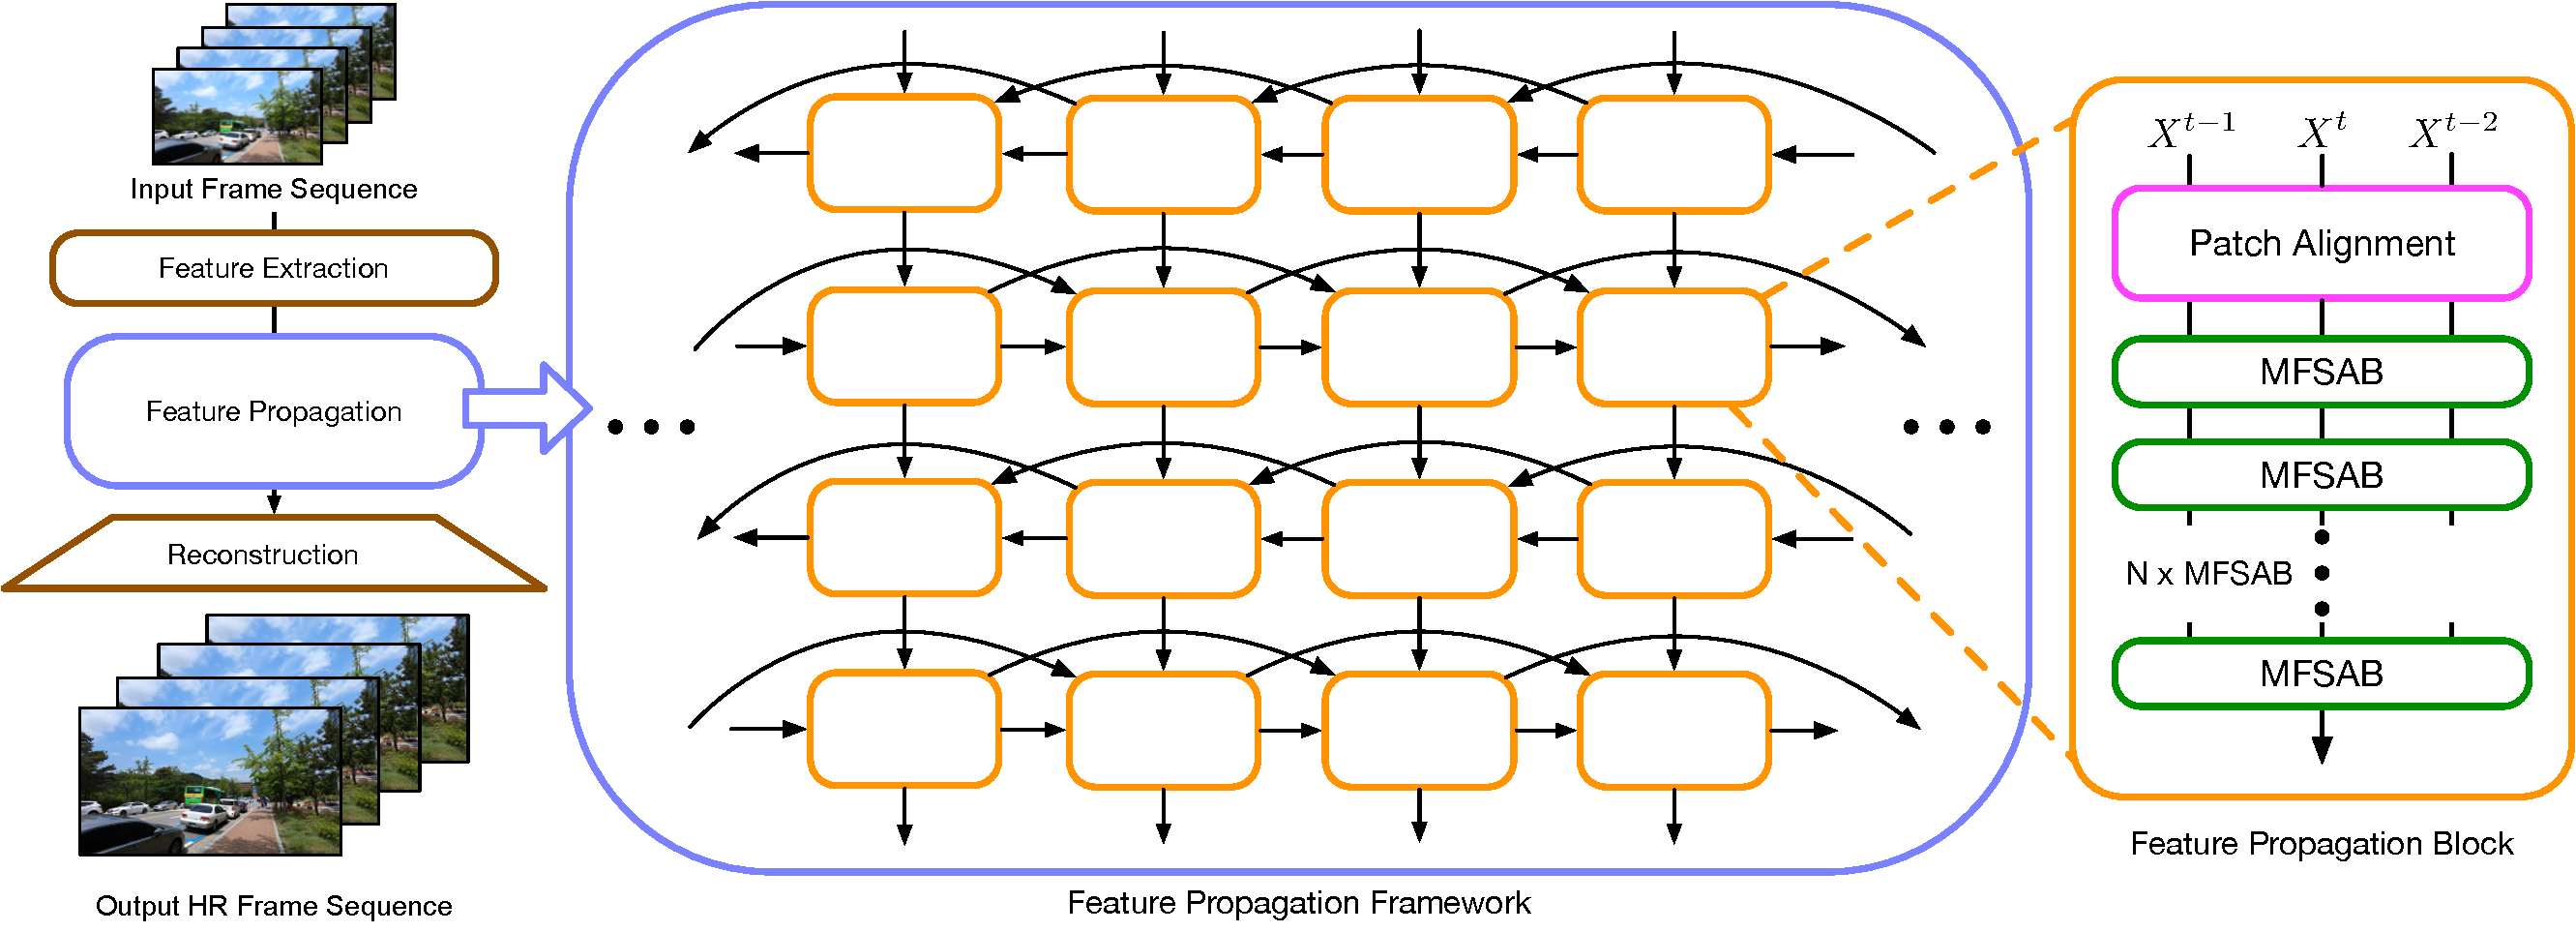
\includegraphics[width=\linewidth]{19.pdf}
	\caption{循环架构的 VSR Transformer}
\end{figure*}

\begin{table*}[!htbp]
  \small
  \centering
  \caption{Quantitative comparison (PSNR$\uparrow$ and SSIM$\uparrow$) on the REDS4 dataset, Vid4, Vimeo-90K-T dataset for $4\times$ VSR task. \textcolor{red}{Red} indicates the best and \textcolor{blue}{blue} indicates the second best performance (best view in color) in each group of experiments.}
   \label{tab:BI-all:supp}
  \vspace{1mm}
  \resizebox{\textwidth}{!}{
  \begin{tabular}{l|c|c||cc|cc|cc}
    \toprule
    \multirow{2}{*}{Method} &  Frames & Params & \multicolumn{2}{c|}{REDS4} & \multicolumn{2}{c|}{Vimeo-90K-T} & \multicolumn{2}{c}{Vid4}\\
    & REDS/Vimeo & (M) & PSNR & SSIM & PSNR & SSIM & PSNR & SSIM \\
    \midrule
    Bicubic                     & -/-  & - &   26.14 & 0.7292  &  31.32 & 0.8684  &   23.78 & 0.6347 \\
    RCAN   & -/- & -  & 28.78 & 0.8200   &  35.35 & 0.9251  &   25.46 & 0.7395 \\
    SwinIR & -/- & 11.9  & 29.05 & 0.8269  & 35.67 & 0.9287  & 25.68 & 0.7491\\
    \midrule
    TOFlow    &       5/7 & - & 27.98 & 0.7990  & 33.08 & 0.9054  & 25.89 & 0.7651\\
    DUF       &   7/7  & 5.8 &  28.63 & 0.8251  & - & - & 27.33 & 0.8319 \\
    PFNL         &   7/7  & 3.0 &  29.63 & 0.8502  & 36.14 & 0.9363 & 26.73 & 0.8029 \\
    RBPN         &   7/7  & 12.2 &  30.09 & 0.8590  & 37.07 & 0.9435 & 27.12 & 0.8180 \\
    EDVR    &   5/7 & 20.6 & 31.09 & 0.8800  & 37.61 & 0.9489 & 27.35 & 0.8264 \\
    MuCAN    &       5/7  & - & 30.88 & 0.8750  & 37.32 & 0.9465 &  - & - \\
    VSR-T    &     5/7 & 32.6 & 31.19 & 0.8815 & 37.71 & 0.9494  & 27.36 & 0.8258  \\
    PSRT-sliding &  5/- & 14.8 & 31.32 & 0.8834 & - & - & - & -\\
    \midrule
    VRT  &  6/- & 30.7 & \textcolor{blue}{31.60} & \textcolor{blue}{0.8888} & - & - & - & - \\
    PSRT-recurrent &  6/- & 10.8 & \textcolor{red}{31.88} & \textcolor{red}{0.8964} & - & - & - & -\\
    \midrule
    BasicVSR & 15/14 & 6.3 & 31.42 & 0.8909 & 37.18 & 0.9450 & 27.24 & 0.8251\\
    IconVSR &  15/14 & 8.7 & 31.67 & 0.8948 & 37.47 & 0.9476 & 27.39 & 0.8279 \\
    BasicVSR++ &  30/14 & 7.3  & 32.39 & 0.9069 &  37.79 & 0.9500 & 27.79 & 0.8400\\
    TTVSR & 50/28&6.8&32.12&0.9021&37.92&0.9526&\textcolor{red}{28.40}&\textcolor{red}{0.8643}\\
    VRT  &  16/7 & 35.6 & 32.19 & 0.9006 & \textcolor{blue}{38.20} & \textcolor{blue}{0.9530} & 27.93 & 0.8425\\
    RVRT  & 30/14 &  10.8 & \textcolor{red}{32.75} & \textcolor{red}{0.9113} & 38.15 & 0.9527 & 27.99 & 0.8462 \\
    % PSRT-recurrent  &  16/7 & 13.4 & \textcolor{blue}{32.72} & \textcolor{blue}{0.9106} & 38.15 & 0.9529 &\textcolor{red}{27.93}& \textcolor{red}{0.8489}\\
    PSRT-recurrent  &  16/14 & 13.4 & \textcolor{blue}{32.72} & \textcolor{blue}{0.9106} & \textcolor{red}{38.27} & \textcolor{red}{0.9536} &\textcolor{blue}{28.07}& \textcolor{blue}{0.8485}\\
    \bottomrule
  \end{tabular}}
\end{table*}
